\documentclass[12pt]{report}

\setlength\parindent{0cm}

%------------------- declaring packages---------------------------------


% styling and graphics-based

\usepackage{graphicx} 
\usepackage{emptypage}
\usepackage[a4paper,
left=3cm,
right=3cm,
top=3cm,
bottom=3cm]{geometry}
\usepackage[percent]{overpic}
\usepackage{setspace}
\usepackage{pgf}
\usepackage{pgffor}
\usepackage{svg}
\usepackage{xcoffins}
\usepackage{xcolor}
\usepackage{caption}
\usepackage{changepage}
\usepackage{fontspec}
\setmainfont{Arial}

\doublespacing

%define colors
% Define custom colors
\definecolor{blueBase}{RGB}{70,130,180}
\definecolor{blueLeaf}{RGB}{135,206,250}

\definecolor{greenBase}{RGB}{34,139,34}
\definecolor{greenLeaf}{RGB}{144,238,144}

\definecolor{orangeBase}{RGB}{255,140,0}
\definecolor{orangeLeaf}{RGB}{255,200,120}

\definecolor{purpleBase}{RGB}{138,43,226}
\definecolor{purpleLeaf}{RGB}{186,85,211}

\definecolor{redBase}{RGB}{178,34,34}
\definecolor{redLeaf}{RGB}{240,128,128}

\definecolor{grayBase}{RGB}{105,105,105}
\definecolor{grayLeaf}{RGB}{169,169,169}

\definecolor{lightblue}{RGB}{225,245,254}
\definecolor{highlightblue}{RGB}{144,202,249}

\definecolor{lightgray}{RGB}{240,240,240}
\definecolor{highlightgray}{RGB}{200,200,200}

\definecolor{darkgreenMW}{RGB}{0, 170, 0} % or choose your own color
\definecolor{lightgreenMW}{RGB}{144,238,144}

% for figures and tables

% figures:
\usepackage{subcaption}
\renewcommand{\thesubfigure}{\Alph{subfigure}}
\usepackage{forloop}
\newcounter{subfigurenumber}
\newcommand{\subplot}[5]{%
  \begin{subfigure}[t]{1\textwidth}
    \centering
    \includegraphics[#2]{#3}
    \phantomcaption\label{sub0:#5}
  \end{subfigure}
  \forloop{subfigurenumber}{1}{\value{subfigurenumber} < #1}{%
    \parbox{0pt}{\phantomsubcaption\label{sub\arabic{subfigurenumber}:#5}}
  }
  \vspace{-0.8cm}
  \caption{#4}\label{#5}
}
% Define subplot with overpic and manual label positioning
\newcounter{customsubfig}
\newcommand{\customsubplot}[8]{%
  \begin{subfigure}[t]{1\textwidth}
    \centering
    \begin{overpic}[width=#2, trim=#3, clip]{#4}
        \put(#5){\large\text{(A)}}
        \put(#6){\large\text{(B)}}
        \phantomcaption\label{sub0:#7}%
    \end{overpic}
\end{subfigure}
\forloop{customsubfig}{1}{\value{customsubfig} < #1}{%
    \parbox{0pt}{\phantomsubcaption\label{sub\arabic{customsubfig}:#7}}
  }
    \vspace{-0.8cm}  
    \caption{#8}
    \label{#7}
}
\usepackage[export]{adjustbox}
\usepackage{wrapfig}
\usepackage{rotating}
\usepackage{lscape}
\usepackage{tikz}
\usetikzlibrary{arrows.meta, positioning, shapes.geometric, 3d, calc}
\usepackage{pgfmath-xfp}
\usepackage{tikz-3dplot}
\tikzset{plane/.style n args={3}{insert path={%
#1 -- ++ #2 -- ++ #3 -- ++ ($-1*#2$) -- cycle}},
unit xy plane/.style={plane={#1}{(1,0,0)}{(0,1,0)}},
unit xz plane/.style={plane={#1}{(1,0,0)}{(0,0,1)}},
unit yz plane/.style={plane={#1}{(0,1,0)}{(0,0,1)}},
get projections/.style={insert path={%
let \p1=(1,0,0),\p2=(0,1,0)  in 
[/utils/exec={\pgfmathtruncatemacro{\xproj}{sign(\x1)}\xdef\xproj{\xproj}
\pgfmathtruncatemacro{\yproj}{sign(\x2)}\xdef\yproj{\yproj}
\pgfmathtruncatemacro{\zproj}{sign(cos(\tdplotmaintheta))}\xdef\zproj{\zproj}}]}},
pics/unit cube/.style={code={
\path[get projections];
\draw (0,0,0) -- (1,1,1);
\ifnum\zproj=-1
 \path[3d cube/every face,3d cube/xy face,unit xy plane={(0,0,0)}]; 
\fi
\ifnum\yproj=1
 \path[3d cube/every face,3d cube/yz face,unit yz plane={(1,0,0)}]; 
\else
 \path[3d cube/every face,3d cube/yz face,unit yz plane={(0,0,0)}]; 
\fi
\ifnum\xproj=1
 \path[3d cube/every face,3d cube/xz face,unit xz plane={(0,0,0)}]; 
\else
 \path[3d cube/every face,3d cube/xz face,unit xz plane={(0,1,0)}]; 
\fi
\ifnum\zproj>-1
 \path[3d cube/every face,3d cube/xy face,unit xy plane={(0,0,1)}]; 
\fi
}},
3d cube/.cd,
xy face/.style={fill=blue!10},
xz face/.style={fill=blue!20},
yz face/.style={fill=blue!30},
num cubes x/.estore in=\NumCubesX,
num cubes y/.estore in=\NumCubesY,
num cubes z/.estore in=\NumCubesZ,
num cubes x=1,num cubes y/.initial=1,num cubes z/.initial=1,
cube scale/.initial=0.9,
every face/.style={draw,very thick},
/tikz/pics/.cd,
cube array/.style={code={%
 \tikzset{3d cube/.cd,#1}
 %\typeout{\NumCubesX,\NumCubesY,\NumCubesZ}
  \path[get projections];
  \ifnum\yproj=1
   \def\LstX{1,...,\NumCubesX}
  \else 
   \ifnum\NumCubesX>1
    \pgfmathtruncatemacro{\NextToLast}{\NumCubesX-1}
    \def\LstX{\NumCubesX,\NextToLast,...,1}
   \else
    \def\LstX{1}   
   \fi 
  \fi
  \ifnum\xproj=-1
   \def\LstY{1,...,\NumCubesY}
  \else 
   \ifnum\NumCubesY>1
    \pgfmathtruncatemacro{\NextToLast}{\NumCubesX-1}
    \def\LstY{\NumCubesY,\NextToLast,...,1}
   \else
    \def\LstY{1}   
   \fi 
  \fi
  \ifnum\zproj=1
   \def\LstZ{1,...,\NumCubesZ}
  \else 
   \ifnum\NumCubesZ>1
    \pgfmathtruncatemacro{\NextToLast}{\NumCubesX-1}
    \def\LstZ{\NumCubesZ,\NextToLast,...,1}
   \else
    \def\LstZ{1}   
   \fi 
   \def\LstZ{\NumCubesZ,\NextToLast,...,1}
  \fi
  \foreach \X in \LstX
  {\foreach \Y in \LstY
   {\foreach \Z in \LstZ
    {
    \ifnum\X=4
      \ifnum\Y=2
        \path (\X-\NumCubesX/2-1,\Y-\NumCubesY/2-1,\Z-\NumCubesZ/2-1)
          pic[scale=\pgfkeysvalueof{/tikz/3d cube/cube scale},
               3d cube/.cd,
               xy face/.style={fill=red!10},
               xz face/.style={fill=red!20},
               yz face/.style={fill=red!30}]{unit cube};
      \else
        \path (\X-\NumCubesX/2-1,\Y-\NumCubesY/2-1,\Z-\NumCubesZ/2-1)
          pic[scale=\pgfkeysvalueof{/tikz/3d cube/cube scale}]{unit cube};
      \fi
    \else
      \path (\X-\NumCubesX/2-1,\Y-\NumCubesY/2-1,\Z-\NumCubesZ/2-1)
        pic[scale=\pgfkeysvalueof{/tikz/3d cube/cube scale}]{unit cube};
    \fi
  }}
  } 
}}
}
% tables:
\usepackage{tabularx,ragged2e,booktabs,caption}
\usepackage{multicol,tabularx,capt-of}
\usepackage{hhline}
\usepackage{multirow}
\usepackage{array}
\usepackage[edges]{forest}


% for math equations

\usepackage{amssymb}
\usepackage{float}
\usepackage{verbatim}
\usepackage{amsmath} 
\usepackage{amsthm}   


% for acronyms and glossaries

\usepackage{acronym}
\usepackage{glossaries}
\usepackage{placeins}

% for hyperlinks

\usepackage[round]{natbib}
\usepackage[colorlinks = true,
            linkcolor = black,
            urlcolor  = black,
            citecolor = black,
            anchorcolor = black]{hyperref}
\newcommand{\figref}[1]{\hyperref[#1]{(Fig.~\ref*{#1})}}
\newcommand{\tabref}[1]{\hyperref[#1]{(Tab.~\ref*{#1})}}

\usepackage{cleveref}
% Make URL links (like DOIs or website links) use Arial
\usepackage{url}
\renewcommand{\UrlFont}{\fontspec{Arial}}

\usepackage{sectsty}
\allsectionsfont{\bfseries}
\chapterfont{\centering\Large}
\sectionfont{\normalsize}
\subsectionfont{\normalsize}


\usepackage [english]{babel}
\usepackage [autostyle, english = british]{csquotes}
\MakeOuterQuote{"}

% header formatting

\usepackage{layout}
\usepackage{fancyhdr}

\fancypagestyle{custompagestyle}{%
    \fancyhf{}
    \fancyfoot[R]{\thepage}
}

\fancypagestyle{noheaderfooter}{%
    \fancyhf{} % Clear header and footer
    \renewcommand{\headrulewidth}{0pt} % Remove header line
}
\usepackage{titlesec}  % Import titlesec for custom chapter formatting

% Remove "Chapter" and display number inline with title
\renewcommand{\thechapter}{\arabic{chapter}}  % Only display chapter number
\titleformat{\chapter}[hang]{\normalfont\Huge\bfseries\centering}
{\thechapter}{1em}{}

\titlespacing*{\chapter}{0pt}{-50pt}{20pt} 

%appendix formatting
\usepackage{appendix}

%footer formatting

\interfootnotelinepenalty=10000

\usepackage{epstopdf}

\def\cx{.85} % relative size of cube vs grid unit
\newcommand{\cube}[4][black]{
  \fill[#1!20] (#2,#3,#4) -- (#2+\cx,#3,#4) -- (#2+\cx,#3+\cx,#4) -- (#2,#3+\cx,#4) -- cycle;
  \fill[#1!10] (#2,#3+\cx,#4) -- (#2,#3+\cx,#4-\cx) -- (#2+\cx,#3+\cx,#4-\cx) -- (#2+\cx,#3+\cx,#4) -- cycle;
  \fill[#1!30] (#2+\cx,#3,#4) -- (#2+\cx,#3+\cx,#4) -- (#2+\cx,#3+\cx,#4-\cx) -- (#2+\cx,#3,#4-\cx) -- cycle;
}

% specify files to use, especially useful if you want to build only one chapter due to build time
%\includeonly{material_methods}

%----------------------------begin document-------------------------------
\setcounter{secnumdepth}{2}  % Chapters and sections are numbered
\counterwithout{figure}{chapter}
\counterwithout{table}{chapter}
\counterwithout{equation}{chapter}

\begin{document}

%\frontmatter
\pagenumbering{roman}

\newgeometry{top=0cm, bottom=3cm, left=1cm, right=1cm}
\begin{titlepage}
	\begin{minipage}{0.3\textwidth}
		\begin{flushleft}
			\includegraphics[height=3cm]{Figures/logos/logo_cob.png} % Replace with your left logo
		\end{flushleft}
	\end{minipage}
	\hfill
	\raisebox{-17ex}{\begin{minipage}{0.3\textwidth}
			\begin{center}
				\includegraphics[height=4cm, trim=0.5cm 0 0 0]{Figures/logos/logo_imbrsea.png} % Replace with your center logo
			\end{center}
		\end{minipage}}
	\hfill
	\begin{minipage}{0.3\textwidth}
		\begin{flushright}
			\includegraphics[height=5.5cm]{Figures/logos/logo_ghent.png} % Replace with your right logo
		\end{flushright}
	\end{minipage}

	% Move logos closer to top margin
	\vspace{2cm}

	% Title of the Thesis
	\begin{center}
		{\LARGE \textbf{Spatio-temporal fishing risk of large pelagic fish in the Mediterranean Sea}}\\[1.5cm]

		\textbf{Master Thesis}\\
		\textbf{Tom Leven}\\
		Submitted on \today\\[1.5cm]

		% Department and Institute information
		At the Faculty of Sciences\\ \textbf{Ghent University}\\[1.5cm]

		Main supervisor: Dr. Pilar Tugores\textsuperscript{1}\\ Co-supervisors: Dr. Diego
		Alvarez-Berastegui\textsuperscript{1} \& Dr. Miguel Cabanellas-Reboredo\textsuperscript{1}\\[1cm]

		\textsuperscript{1} \small{Centro Oceanográfico de Illes Balears (COB-IEO), CSIC\@.\\Moll de Ponent s/n, 07015 Palma de Mallorca, Illes Balears (Spain)}

	\end{center}

\end{titlepage}
\restoregeometry
\newpage
\thispagestyle{empty}
\vspace*{\fill}
\begin{center}
	\textit{‘No data can be taken out of this work without prior approval of the thesis main supervisor(*)’}
\end{center}
\vspace*{\fill}

\chapter*{Executive Summary}

The executive summary goes here.

\addcontentsline{toc}{chapter}{Executive Summary}

\chapter*{Abstract}

Abstract goes here.

\addcontentsline{toc}{chapter}{Abstract}

\tableofcontents{}

%\listoftables{}

%\listoffigures{}

\thispagestyle{noheaderfooter}
\cleardoublepage

\pagenumbering{arabic}
\setcounter{page}{1}

\chapter{Introduction}

\begin{itemize}
    \item Delineating fishing grounds essential for fisheries management
    \item Traditional tools and shortcomings, logbooks, VMS (resolution, ping rate etc.)
    \item AIS as promising tool to understand fisheries dynamics for example to estimate fishing effort or to aid in fisheries governance (MCS)
    \begin{itemize}
        \item Explain how AIS works
    \end{itemize}
    \item Limitations of AIS
    \item Conservation issues in Mediterranean, highly migratory species
    \begin{itemize}
        \item New approach in ICCAT to go towards climate informed fisheries
        \item TunaMed Observatory
        \item Monitor changes in spatio-temporal distribution essential
        \item Develop indicators for habitat changes due to climate change but also indicators for human pressures like fishing
    \end{itemize}
    \item BFT collapse and exploitation history, tuna farms
    \item Countries report coarse spatial data to ICCAT, if any
    \item AIS allows fine-scale analysis of spatio-temporal changes
    \item Metiers for each species, when they are fished, how they migrate
    \item Research questions:
    \begin{itemize}
        \item Where and when is fishing activity for large pelagic species most intense and has this changed over time from 2015-2024?
        \item What are the seasonal patterns of fishing activity by gear type and do they differ interannually?
        \item To what extent does AIS capture the full scope of fishing activity in the Mediterranean?
        \item What is the spatial relationship between fishing hours and environmental features such as distance to port, and bathymetry
              and how does this differ between the two gear types?
        \item How: Fishing hours data from GFW etc.

    \end{itemize}
\end{itemize}



\chapter{Material and Methods}

\section{Data sources}
\subsection{Fishing hours}
Data on fishing hours was obtained from Global Fishing Watch (GFW). This non-profit organization provides a global dataset of estimated fishing activity
derived from AIS data \citep{gfw_dataset}. 
They process data from over 190,000 unique AIS transmitters, each assigned a unique Maritime Mobile Service Identity (MMSI).
These AIS devices broadcast a vessel's location as frequently as every 2 seconds \citep{kontasvesselupdate, taconet2019global}. Along with the exact location,
each AIS transmission includes a timestamp, speed, and heading of the vessel. GFW then analyses these positional data points, to infer fishing activity, via two 
different Convolutional Neural Networks (CNN's), which are described in detail in \cite{Kroodsma18}. 

\bigskip

A first CNN classifies fishing vessels into one of sixteen fishing gear categories \figref{fig:vessel_classification} and 
predicts vessel characteristics such as length, tonnage, and engine power. This deep-learning model is trained on
a dataset of vessels matched to official vessel registries which are \textit{known} fishing vessels. Vessels without
gear information in the registries used are assigned a gear if their movement patterns resemble those of a known
vessel class. A second CNN classifies every obtained AIS position as either fishing or non-fishing based on characteristic fishing movement (\citeauthor{Kroodsma18}, \citeyear{Kroodsma18}; Fig.~\ref{fig:workflow}). 
These individual fishing events are then aggregated into grid cells spanning either 0.1° or 0.01° on a side. For the present analysis, 0.1° resolution was chosen,
covering the study area (Mediterranean Sea; Fig~\ref{fig:study_area}) in sufficient detail.

\bigskip

Unique vessels are identified based on their MMSI number and the dataset contains information
on the vessel's registration and flag country. The gear class estimated by the CNN is also compared with the information
from different vessel registries, such as the EU fleet register or the ICCAT record of vessels. In case the derived vessel class
does not match to the one in the registry, GFW assigns the broadest gear type that allows for agreement. If for example,
a vessel is registered as a purse seiner but is inferred to be a tuna purse seiner, it would ultimately be assigned to the
purse seiner class \figref{fig:vessel_classification}.
\medskip
\begin{figure}[htbp]
\centering
\resizebox{\textwidth}{!}{%
\begin{forest}
    [Fishing, fill=grayBase, for tree={grow=east,
        draw,
        rounded corners,
        minimum height=1.2em,
        text width=4cm,
        align=center,
        parent anchor=east,
        child anchor=west,
        edge path={\noexpand\path [draw, \forestoption{edge}]
            (!u.parent anchor) -- +(5pt,0) |- (.child anchor)\forestoption{edge label};},
        l sep+=10pt,
        s sep+=10pt}
        [Squid Jigger, fill=grayLeaf]
        [Drifting Longlines, fill=grayLeaf]
        [Pole And Line, fill=grayLeaf]
        [Trollers, fill=grayLeaf]
        [Fixed Gear, fill=blueBase
            [Pots And Traps, fill=blueLeaf]
            [Set Longlines, fill=blueLeaf]
            [Set Gillnets, fill=blueLeaf]]
        [Trawlers, fill=grayLeaf]
        [Dredge Fishing, fill=grayLeaf]
        [Seiners, fill=greenBase
            [Purse Seines, fill=greenBase
                [Tuna Purse Seines, fill=greenLeaf]
                [Other Purse Seines, fill=greenLeaf]]
            [Other Seines, fill=greenLeaf]]]
    \end{forest}
} % end resizebox
\medskip
\caption{Hierarchy of fishing gears recognised by GFW}
\label{fig:vessel_classification}
\end{figure}

\subsection{ICCAT catch data}
Data on catches of large-pelagic species in the Mediterranean is openly available from the International Commission for the 
Conservation of Atlantic Tunas (ICCAT). Nominal catch data was obtained for the period 2015-2023 and filtered for the major 
large pelagic species like tunas and billfishes \citep{iccat_catches}.


\subsection{Bluefin Tuna vessels}
Individual purse seine vessels that were assigned a bluefin tuna quota for 2024 were obtained from the corresponding national notices. In France,
quotas are allocated and published by the \cite{registry_france}. In Spain,
by the \cite{registry_spain} and in Italy by the \cite{registry_italy}. These countries were chosen exemplary because in the period from 2015 to 2023,
they made up more than half of the total landings of BFT for all contracting parties to ICCAT, of which close to 90\% are fished with purse seine nets \citep{iccat_bft_summary}.
Since the national notices did not contain the vessels MMSI number (which is the identifier used by GFW), the vessel names and registration numbers were
cross-referenced with the Europan Fleet Register to obtain it \citep{eu_fleet_register}. 


\section{Data filtering}
All data filtering was conducted using R (v4.4.1; \citeauthor{r_language}, \citeyear{r_language}) within the RStudio environment \citep{rstudio}.
The GFW dataset was first cropped and adjusted to a shapefile of the Mediterranean Sea \figref{fig:med}, obtained from the General Fisheries
Commission for the Mediterranean (GFCM). Subsequent filtering was based on the assigned gear type and GFW registry
information. Only entries with the gear type drifting longlines or tuna purse seines, and that were registered with
ICCAT were retained \figref{fig:workflow}. These gear types were chosen as they are the main \textit{metiers} involved in the exploitation of large-pelagic species in the Mediterranean.
Since 2015, on average, 95\% of BFT's, and 99\% of albacore tunas are caught using either longlines or purse seine nets and close to 100\% of swordfish catches use longlines \citep{iccat_bft_summary,iccat_alb_summary,iccat_swo_summary}
The GFW dataset is available from the year 2012 until 2024. However, only entries from 2015 were retained, in order to avoid masking \textit{real} fishing dynamics with the increase in
adoption of AIS devices, which only became mandatory in the EU in 2014 for all vessels > 15 m in length \citep{ec2011directive}. It is estimated however, that in the Mediterranean the EU fishing fleet >15 m is 100\% equipped with AIS since 2018 \citep{taconet2019global}.

\begin{figure}[htp]
      \begin{center}
        \begin{tikzpicture}[
            node distance=0.9cm,
            gfwbox/.style={rectangle, draw, rounded corners, text width=4.2cm, align=center, minimum height=1cm, fill=lightblue},
            yourbox/.style={rectangle, draw, rounded corners, text width=4.2cm, align=center, minimum height=1cm, fill=lightgray},
            gfwfinal/.style={rectangle, draw, rounded corners, text width=4.2cm, align=center, minimum height=1cm, fill=highlightblue},
            yourfinal/.style={rectangle, draw, rounded corners, text width=4.2cm, align=center, minimum height=1cm, fill=highlightgray},
            gfwheader/.style={font=\bfseries\large, text width=5.5cm, align=center},
            yourheader/.style={font=\bfseries\large, text width=4.2cm, align=center},
            arrow/.style={-{Stealth}, thick}
        ]
        
        % GFW Header (wider)
        \node[gfwheader] (gfwheader) at (0,0) {Global Fishing Watch Processing};
        %GFW logo
        \node[anchor=north west] at ([xshift=-1.5cm,yshift=2cm]gfwheader.north east) {\includegraphics[width=3cm]{Figures/logos/GFW_logo.png}};
        % GFW Steps
        \node[gfwbox, below=of gfwheader] (raw) {Raw AIS positions};
        \node[gfwbox, below=of raw] (cnn1) {CNN 1: Vessel classification};
        \node[gfwbox, below=of cnn1] (cnn2) {CNN 2: Detect fishing activity};
        \node[gfwfinal, below=of cnn2] (grid) {Gridded fishing hours per MMSI/trip};
        
        \draw[arrow] (raw) -- (cnn1);
        \draw[arrow] (cnn1) -- (cnn2);
        \draw[arrow] (cnn2) -- (grid);
        
        % Your Workflow Header
        \node[yourheader, right=3cm of gfwheader] (yourheader) {Filtering Steps};
        % R Logo in top-right corner
        \node[anchor=north west] at ([xshift=-1cm,yshift=1.3cm]yourheader.north east) {\includegraphics[width=1.5cm]{Figures/logos/R_logo.png}};

        % Your Steps
        \node[yourbox, below=of yourheader] (crop) {Crop to Mediterranean Sea area};
        \node[yourbox, below=of crop] (gear) {Gear types: \\ Drifting longlines \& tuna purse seines};
        \node[yourbox, below=of gear] (registry) {GFW registry \\ includes ICCAT};
        \node[yourbox, below=of registry] (national) {Manually adding known purse seiners \\ based on national quota allocation};
        \node[yourbox, below=of national] (port) {Remove cells <1 km \\ from port};
        \node[yourfinal, left=2cm of port] (final) {Final dataset used};
        
        \draw[arrow] (crop) -- (gear);
        \draw[arrow] (gear) -- (registry);
        \draw[arrow] (registry) -- (national);
        \draw[arrow] (national) -- (port);
        \draw[arrow] (port) -- (final.east);
        
        % Connector from GFW to your steps
        \draw[arrow] (grid.east) -- ++(0.5,0) |- (crop.west);
        
        \end{tikzpicture}
        \end{center}        
\caption{Global Fishing Watch data processing pipeline and filtering steps to obtain the final dataset used in this study. CNN = Convolutional Neural Network}
\label{fig:workflow}
\end{figure}

\medskip

In case of the tuna purse seiners, these filtering steps also removed some vessels which are known to be fishing for bluefin tuna based on 
national quota allocations (obtained for Spain, France, and Italy). These vessels were
removed by the filtering steps either because GFW assigns them a different gear type, or they are not present in the
registry information from ICCAT that GFW uses. For the present analysis, these vessels were thus, manually included after comparison with the information from the national
vessel registries.

\medskip

Irregular vessel movement patterns occurring in or near ports can falsely resemble fishing activity and should therefore be excluded when estimating fishing effort. 
These movements include cruising towards the harbour to land catches or vessel maintenance \citep{souza}. Thus,
to remove these areas from the analysis, the points inside the 1 km boundary around ports were removed. Distance from port was determined based on a dataset from 
GFW, which contains anchorages that are either known ports, or that contained at least 20 unique stationary vessels since 2012 \citep{gfw_distance}. 

\section{Data analysis}
To identify persistent hotspot areas throughout the one decade study time and analyse spatio-temporal trends, the Emerging Hotspot Analysis (EHA) tool
was used in ArcGIS Pro \citep{arcgis}. For this, multidimensional netCDF (network common data form) files of the fishing hours data were generated after curation and filtering in R, using
the \textit{terra} package (v1.8.18; \citeauthor{terra_package}, \citeyear{terra_package}). Subsequently, this data was read in as multidimensional raster files in ArcGIS Pro, with the
dimensions corresponding to longitude, latitude and time. Data was aggregated annually, using the sum of fishing hours per year for each cell.
From this, a space-time cube, which is the input required for the EHA tool, was created (Fig.~\ref{fig:cube}A).

\begin{figure}[H]
\begin{subfigure}{0.45\textwidth}
    \tdplotsetmaincoords{60}{45} 
    % the first argument cannot be larger than 90
    \begin{tikzpicture}[tdplot_main_coords, line join=round, 3d cube/.cd,
        num cubes x=4, num cubes y=4, num cubes z=4]
        \node[font=\large] at (-8,1) {(A)};
        \path pic {cube array={}};

        Longitude, Latitude, Time) aligned with cube edges
        % Make sure you're inside this scope:
        \begin{scope}[tdplot_main_coords]
            
            % Arrow: Longitude (X-axis): from left-bottom-front to middle-bottom-front
            \draw[->, thick, orangeBase]
            (-2.5, -2.5, -2.5) -- (3, -3, -2)
            node[midway, below, sloped] {Longitude};
            
            % Arrow: Latitude (Y-axis): from middle-bottom-front to right-bottom-front
            \draw[->, thick, grayLeaf]
            (3, -3, -2) -- (3, 2, -2)
            node[midway, below, sloped] {Latitude};
            % Arrow: Time (Z-axis): from bottom-left to top-left
            \draw[->, thick, greenBase]
            (-2.5, -2.5, -2.5) -- (-2, -3, 2)
            node[midway, left] {\shortstack{Time\\(Years)}};

            \draw[->, thick, red!70]
            (2,-1.2, 2.4)..controls(0,0.5,2.2)..(0.7,0.7,3.5);
            
            \node[text=black] at (1,1,3.9) {Time series bin};

        \end{scope}
        
    \end{tikzpicture}
\end{subfigure}
\hspace{1.5cm}
    \begin{subfigure}{0.45\textwidth}
        \centering
        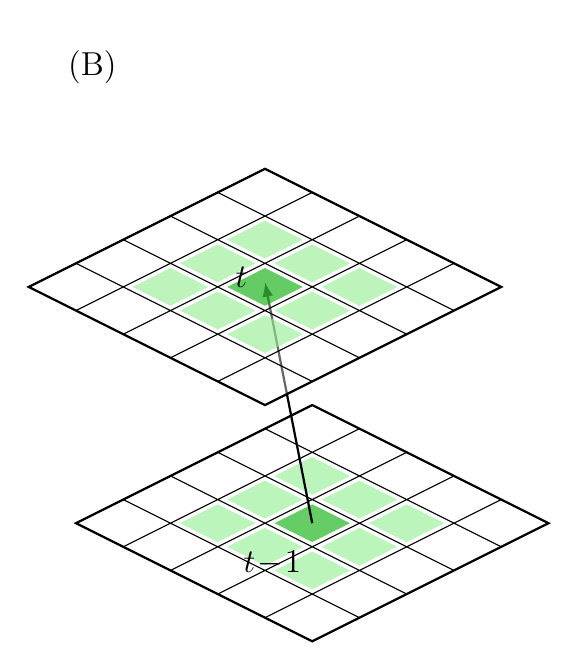
\begin{tikzpicture}[scale=.6, every node/.style={minimum size=1cm}]
        \node[anchor=north west, font=\large] at (-4.5,8) {(B)};
        % Define grid and insets
        \def\gridsize{5}
        \def\cellsize{1}
        \def\inset{0.1} % amount to inset the fill from each side
        
        % Function to draw filled cell with inset
        \newcommand{\fillcell}[3]{
            \fill[#3, fill opacity = 0.6] (#1+\inset,#2+\inset) rectangle (#1+1-\inset,#2+1-\inset);
            }
            
        % === First Grid (lower, 3D perspective) ===
        \begin{scope}[yshift=-5cm, xshift=1cm, every node/.append style={yslant=0.5,xslant=-1}, yslant=0.5, xslant=-1]
            \draw[step=\cellsize, black] (0,0) grid (\gridsize,\gridsize);
            \draw[black, thick] (0,0) rectangle (\gridsize,\gridsize);

  % Center cell
  \fillcell{2}{2}{darkgreenMW}

  % 8-neighbourhood
  \foreach \x/\y in {1/1, 1/2, 1/3, 2/1, 2/3, 3/1, 3/2, 3/3} {\fillcell{\x}{\y}{lightgreenMW}}
\end{scope}

% === Arrow (behind top grid) ===
\coordinate (center_tminus1) at (1,3.5-6); % center of bottom grid
\coordinate (center_t) at (0,2.6);       % center of top grid
\draw[-latex, thick, black] (center_tminus1) -- (center_t);
\node[below left, font=\bfseries\large] at (center_tminus1) {$t\!-\!1$};

% === Second Grid (upper, semi-transparent overlay) ===
\begin{scope}[yshift=0cm, every node/.append style={yslant=0.5,xslant=-1}, yslant=0.5, xslant=-1]
  \fill[white, fill opacity=0.4] (0,0) rectangle (\gridsize,\gridsize);
  \draw[step=\cellsize, black] (0,0) grid (\gridsize,\gridsize);
  \draw[black, thick] (0,0) rectangle (\gridsize,\gridsize);

  % Center cell
  \fillcell{2}{2}{darkgreenMW}

  % 8-neighbourhood
  \foreach \x/\y in {1/1, 1/2, 1/3, 2/1, 2/3, 3/1, 3/2, 3/3} {\fillcell{\x}{\y}{lightgreenMW}}
\end{scope}

% === Annotations ===
\node[font=\bfseries\large] at (-0.5,2.7) {$t$}; % Position manually above the top grid

        \end{tikzpicture}
    \end{subfigure}
\bigskip
\caption{A) Structure of the space-time cube in ArcGIS\@. Each individual cube corresponds to one \textit{neighbourhood bin}, which is the sum of all coloured cells in B. One \textit{time series bin}
corresponds to the same location over time (red).  B) Conceptualization of space-time dependency as implemented in the Emerging Hotspot Analysis tool. One \textit{neighbourhood  bin}
is defined as the cell itself (darkgreen) plus the cells surrounding it (lightgreen), as well as those cells in the previous time step (\(t-1\)).}
\label{fig:cube}
\end{figure}

EHA uses a combination of two statistical methods. First, the Getis-Ord \(G_i^*\) statistic to identify areas where low/high values are spatially clustered \citep{getis_ord}. The null hypothesis
states that the sum of values of location \( i \) and its neighbours, is not significantly different from what would be expected by chance, based on all observations (neighbours are
defined as shown in Fig.~\ref{fig:cube}B). Thus, each \textit{neighbourhood} contains the cell itself, plus all cells contiguous with it via edges and corners at time \(t\) and \(t-1\).
Each neighbourhood is compared to all global observations at the current and preceding time step. Based on the neighbourhood definition,
a binary spatial weight matrix is constructed, where each entry \(w_{i,j}\), is either 1 (if features \(i\) and \(j\) are neighbours) or 0 otherwise. The \(G_i^*\) statistic is then
calculated as:

\begin{equation}
G_i^* = \frac{\displaystyle\sum_{j=1}^{n} w_{i,j} x_j - \bar{X} \displaystyle\sum_{j=1}^{n} w_{i,j}}{S \sqrt{\frac{n \displaystyle\sum_{j=1}^{n} w_{i,j}^2 - \left( \displaystyle\sum_{j=1}^{n} w_{i,j} \right)^2}{n-1}}}
\end{equation}

\bigskip

where \( x_j \) is the value for feature \( j \), 
\( w_{i,j} \) is the spatial weight between feature \( i \) and \( j \), 
and \( n \) is the total number of features. The terms \( \bar{X} \) and \( S \) represent the global mean and standard deviation
of the attribute values, respectively, and are given by:

\begin{equation}
\bar{X} = \frac{\displaystyle\sum_{j=1}^{n} x_j}{n}
\end{equation}
\medskip
\begin{equation}
S = \sqrt{\frac{\displaystyle\sum_{j=1}^{n} x_j^2}{n} - \left(\bar{X}\right)^2}
\end{equation}\\

The implementation of \(G_i^*\) in the EHA tool also applies a False Discovery Rate (FDR) correction to account for multiple testing and spatial dependency in the data.
This approach is preferred over methods like Bonferroni correction, which only accounts for multiple testing, as FDR is less conservative and less likely to miss true 
positives \citep{fdr_correction}. EHA is thus, a spatio-temporal extension of the \(G_i^*\) statistic, as it extends each cell not only to its spatial but
also to the temporal neighbours.

\bigskip

Second, EHA applies the Mann-Kendall trend test to evaluate whether there is a monotonic upward or downward trend in each time series bin \citep{mann1945nonparametric,kendall1990rank}.
The non-parametric Mann-Kendall statistic \(S\) analyses each time series bin. It ranks and compares each point \( x_i \) (for \( i = 1, 2, \ldots, n-1 \)) 
to all subsequent points \( x_j \) (for \( j = i+1, i+2, \ldots, n \)) and is given by (\citeauthor{kendall1990rank}, \citeyear{kendall1990rank}, Section 1.9)

\begin{equation}
S = \sum_{i=1}^{n-1} \sum_{j=i+1}^{n} \text{sign}(x_j - x_i)
\end{equation}

\bigskip

Where the sign function is defined as:

\begin{equation}
\text{sign}(x_j - x_i) = \text{sign}(R_j - R_i)
\begin{cases}
\phantom{-}1 & x_i < x_j \\
\phantom{-}0 & x_i = x_j \\
  -1 & x_i > x_j
\end{cases}
\end{equation}

\bigskip

and \(R_i\) and \(R_j\) are the ranks of observations \(x_i\) and \(x_j\) of each time series.
Thus, for every time point, it assigns a 1 if the value is higher than the previous one, a 0 if the value is the same, and a -1 if the value is lower. These scores are
then summed for each time series bin and under the null hypothesis of no trend, the value of \(S\) is zero. To assess the significance of \(S\), the variance \(V^*_0\)
can be calculated as (\citeauthor{kendall1990rank}, \citeyear{kendall1990rank}, Section 4.9)

\begin{equation}
    V^*_0 (S) = n(n - 1)(2n + 5) / 18 - \sum_{j=1}^{m} t_j(t_j - 1)(2t_j + 5) /18
\end{equation}

\bigskip

where \(n\) is the total number of observations, and \(m\) the number of groups with tied ranks, each with \(t_j\) tied observations. 


\chapter{Results}

Lorem ipsum dolor sit amet \cite{paolo24satellite}.

\chapter{Discussion}
In this study, the fishing activity targetting large pelagic fishes (LPF) across the Mediterranean
Sea was analysed. Strong spatial and temporal patterns in how fishing is distributed, as well as
regional hotspots were identified. Furthermore, the utility of AIS in monitoring industrial LPF
fleets was shown, while a big gap in the uptake of AIS technology between countries in southern and
northern Mediterranean countries was found.

\section{Main risk areas (hotspots)}
Fishing hotspots and thus, the main risk areas for LPF, aligned with the species' known aggregation
sites, particularly around the Balearic Islands, the Tyrrhenian Sea, the Adriatic Sea, and off the
coasts of Cyprus and Malta. These hotspot regions overlap with key spawning and feeding areas
identified in previous studies \citep{medina_spawning,arocha_2007}. A prime example of this is the
migration of large (>150 kg) bluefin tuna (BFT) from the Atlantic towards their spawning regions in
the Mediterranean between mid-May until mid-July, which drives intense seasonal purse seine
activity \citep{bft_mig_med}. However, some smaller individuals remain resident in the
Mediterranean the whole year-round \citep{cermeno_15_tagging,heinisch_08}. The presence of this
all-year-round stock might explain the extended season of longliners. The spatio-temporal
distribution of the purse seiners around the Balearic Islands, and the Tyrrhenian Sea indicates
that they target known spawning grounds \citep{medina_spawning}. Interestingly, the spawning area
around the Strait of Sicily was not consistently identified as a purse seine hotspot even though
this area is frequented by fleets of up to 5 countries. This is likely because of a lack in the
adoption of AIS by non-EU countries, which is one potential handicap of AIS derived fishing
activity \citep{taconet2019global,paolo24satellite}.

\medskip

The Adriatic Sea appeared to be the most consistent purse seine hotspot identified in our study and
is frequented by purse seiners from Italy and Croatia (Fig.~\ref{fig:seines_hotspots}
and~\ref{fig:seine_effort_countries}). Contrary to the narrow temporal window of the purse seine
activity in the rest of the Mediterranean (which follows the spawning aggregations and the allowed
fishing season) the Adriatic fleet operates in all seasons, particularly vessels flagged to Croatia
(Fig.~\ref{fig:seines_ridge} and~\ref{fig:seine_effort_countries}). This might not only be
explained by ecological aspects like the presence of smaller individuals throughout the whole year,
but also due to socio-economic aspects and the fact that Croatia and Italy are the only countries
permitted to catch individuals < 30 kg for the use in tuna farms (Fig.~\ref{fig:hrv};
\citealp{hrv_farms}).

\medskip

The centroid of the purse seine hotspot around the Balearic Islands showed temporal variability and
moved from the north-west of Ibiza more towards the south and the Mallorca channel
\figref{fig:pss_yearly}. This could relate to the position of a frontal region which has been shown
to be spatially dynamic over time, and important for the spawning location of BFT
\citep{balbin_14,reglero_12}. Other species whose migratory patterns support the fishing activity
found here is swordfish (\textit{Xiphias gladius}). Swordfish in the Mediterranean Sea are
genetically distinct and only show limited migration between there and the Atlantic. Migratory
patterns are highly complex in general and poorly studied within the Mediterranean Sea. Spawning
migration is however linked to thermal fronts, particularly the 24\textdegree C isotherm
\citep{palko1981swordfish,arocha_2007}. Corresponding to this, they spawn from June to August in
areas west of the Balearic Islands until the Strait of Gibraltar, in the Tyrrhenian Sea and the
Strait of Messina, the Levantine Sea, and the Gulf of Taranto in the Ionian Sea (see Fig. 5 in
\citealp{arocha_2007}). They are targeted mainly by the longline fleet and corresponding hotspots
overlapped closely with these spawning areas, particularly in the western Mediterranean and the
Tyrrhenian region.

\medskip

Our analysis did not reveal clear temporal trends within most swordfish longline hotspots. This is
likely due to the use of different types of longlines targeting various species, which are all
analysed together in our study. As a result, we are limited in linking observed patterns within
each hotspot to the specific, dynamic habitat use of individual species, as we were able to do for
the purse seine fishery targeting bluefin tuna around the Balearic Islands.

\medskip

Monitoring the fine-scale spatio-temporal dynamics of the swordfish longline fishery is still
however, particularly valuable because juveniles and adults occupy distinct habitats: juveniles
tend to remain in coastal waters, while adults are more associated with deeper, pelagic zones
\citep{damalas_14_swo}. This spatial segregation by life stage offers an opportunity for more
targeted monitoring and management. AIS data can for example help identify when and where longline
fishing activity occurs close to shore, potentially indicating higher risks of juvenile bycatch.
Such information could be used to assess compliance with existing regulations, guide the
implementation of spatial or seasonal closures, and evaluate whether these are effectively
protecting juvenile habitats. Given that juvenile catch rates were still high prior to the 2017
introduction of a minimum size limit of 100 cm lower jaw fork length, and that discards have since
increased due to undersized individuals being caught, spatially explicit monitoring tools like AIS
could support more adaptive and precise management of the fishery
\citep{iccat_juvenile_catches_swo,iccat_juvenile_swo_ortiz,iccat_swo_discards}.

\medskip

Hotspots in general however, are quite consistent along our study period (2015-2024), and the main
fishing grounds stay the same (Fig.~\ref{fig:dll_yearly} and~\ref{fig:pss_yearly}). This might be
related to the large-scale stability of the spawning and feeding grounds of the LPF targeted. This
should however be closely monitored in the future considering the big impacts of climate change on
the Mediterranean Sea (REF). Tracking fisheries spatially and comparing data between different
years might provide early signs of changes in the distribution of these species, especially when
combined with logbook catch data (e.g., \citealp{campos_ais_logbook}). The clear seasonality of the
purse seine fleet can be attributed to the timing of BFT migration into the Mediterranean and the
implemented seasonal closures and TAC's decided upon by ICCAT, which are usually reached in a very
short amount of time.

\medskip

The fleets investigated in the present study and especially longliners, not only have an important
impact on target species but also on other species caught as bycatch \citep{bycatch_book}, Bycatch
in Mediterranean longline fisheries is a concern for among others, seabirds, pelagic elasmobranchs,
and sea turtles \citep{spain_swo_gear,shark_bycatch,baez_turtles_bycatch}. Drifting longlines for
example are estimated to be responsible for the bycatch of about 27 000 individual sea turtles
annually in the Mediterranean alone \citep{bycatch_book}. The longline hotspots identified here
overlap with estimates of high relative abundance of bycatch species like loggerhead turtles
(\textit{Caretta caretta}; \citealp{dimatteo_turtles}). \cite{bycatch_malta} analysed the longline
fishery around Malta and reported that \textit{Caretta caretta} makes up 40\% of the total catch in
terms of individual animals. Considering very high and increasing trends in the longline activity
in this area, closer monitoring on bycatch rates would be necessary. There is significant interest
from both conservation and fisheries to mitigate bycatch \citep{bycatch_humans} and there have been
recent advances in mitigating turtle bycatch for some fleets through targetted management and/or
changes in the gear used (\citealp{baez_turtles_spain} and ICCAT Reg. 22-12). The results and
methodology employed here, could be a starting point to identify high risk areas overlapping with
important turtle habitat, to better target the deployment of onboard observers. This is just an
example for one species group, but further studies could look into fine-scale spatial overlap
between non-target species and longlines, to better estimate the risk for specific species groups.

\medskip

A significant number of vessels are likely to be missed in our analysis due to inconsistencies
between the vessel registries used by Global Fishing Watch (GFW) and how the gear type is assigned.
Since GFW is assigning a gear class not only based on the registry, but also taking the vessels'
movement into account, there can be discrepancies between them, especially if vessels use multiple
gears over time. This is why we decided to include bluefin tuna purse seiners identified from our
own research based on national vessel registries, irrespective of the gear type assigned by GFW\@.
The national notices are however published by each country in their respective language and are not
easily accessible for cross-country analyses. The
\href{https://www.iccat.int/en/VesselsRecord.asp}{ICCAT record of vessels} contains details on
currently active vessels and their quota allocation, as well as their historic fishing
authorizations for specific species. Further improvements to this resource might be to add historic
quota allocation for each vessel to the downloadable files, and also add information on historic
quotas to the inactive vessel list, which could simplify analyses like this study to obtain a more
complete picture of fishing activity.

\medskip

Since 2018, the usage of VMS is binding for all fishing vessels above 24 m LOA (ICCAT Reg. 18-10)
and fishing vessels above 15 m length overall (LOA) that are authorized to fish species managed by
ICCAT in waters beyond their flag countries jurisdiction. Additionally, all vessels authorized to
fish BFT by ICCAT are required to use VMS and share this data with ICCAT (ICCAT Reg. 21-16). This
data is however, not made public due to concerns about privacy. Incorporating this information into
stock assessments and making it publicly available could however greatly aid in increasing the
transparency of these fisheries that are often linked to Illegal, Unreported, and Unregulated (IUU)
fishing \citep{iccat_bft_summary} (need more citations).

\section{Data caveats}
Although AIS was not originally designed for the estimation of fishing effort and there are some
persistent challenges in deriving fishing effort from these tracking devices, they provide a very
valuable, publicly available source of information for scientists, conservationists and fishery
authorities. Analyses of fine-scale spatial fisheries data derived from AIS have indeed been a
revolution in fisheries science and a great step towards increasing the transparency of all human
activity at sea. However, to advance towards a better application of AIS data for fisheries
monitoring, various improvement could be made. One challenge is the variability in AIS reception,
which depends on a combination of terrestrial, satellite, and dynamic onboard receivers. Coverage
is not uniform, and has changed over time, which can lead to apparent changes in fishing activity
that may reflect improved signal reception rather than actual shifts in effort. GFW is however
working on a dataset that quantifies AIS coverage for each vessels' trip, which will reduce
uncertainty in analysing time series data.

\medskip

AIS data is also biased towards larger vessels (> 15 m) and countries where its use is mandatory.
This can limit its ability to fully represent fishing activity in regions dominated by small-scale
fleets and where fleets without AIS are present, as is the case in the Mediterranean. This bias was
evident for example in the lack of French longline vessels from the Gulf of Lions which are mainly
below 15 m LOA \citep{french_longlines}. Additionally, differences in gear types and fishing
strategies are not always captured by AIS-based models. For example, longliners and purse seiners
measure effort differently (e.g., number of hooks vs.\ number of sets), while GFW’s general fishing
detection model uses fishing hours as a unified metric. This can lead to potential overestimation
of absolute effort, though the geographic accuracy of fishing locations remains high \citep{bias}.

\medskip

Finally, AIS alone cannot distinguish between métiers, which limits species-specific analyses.
Future research could combine AIS with catch or logbook data to estimate catch per unit effort
(CPUE), allowing a more accurate evaluation of fishing operations and thus, resource abundance
\citep{niu_ais_cpue}.

\medskip

The results of this study demonstrate the broad distribution of fishing in almost the whole
Mediterranean Sea and can contribute to the sustainable exploitation of migratory LPF\@. The
methods used here could be combined with other data like log books to get a more detailed
information on changes in relative abundance of target species. This would provide more details on
fishing fleets to management, which is necessary for the implementation of ecosystem-based
management. The areas we identified as fishing hotspots, and potentially also the migratory paths
between them, could be prime targets for management for example to implement seasonal or spatial
closures. \cite{relano_pauly} proposed to protect migratory LPF through \textit{Blue Corridors},
essentially protected areas along the species' migratory pathways. Our findings could help in
identifying these areas. Mapping of the intensity of fishing does also have direct implications for
conservation, as bycatch rates can be quite high for pelagic longliners in the Mediterranean.

\chapter{Conclusion}

Lorem ipsum dolor sit amet, consectetur adipiscing elit \cite{paolo24satellite}.

\chapter{Acknowledgements}

Thank you to.

\bibliographystyle{plainnat}
\bibliography{bibliography}

\begin{appendices}
\renewcommand{\thefigure}{S\arabic{figure}}
\setcounter{figure}{0}

\chapter{Supplementary Material}

Annex 1

\end{appendices}

\end{document}